\documentclass[11pt]{beamer}
\usetheme{Rochester}

\usepackage[utf8]{inputenc}
\usepackage[T1]{fontenc}

\usepackage{url}

\title{WaCC: Architecture}
\subtitle{Distributed (smart) electric charging poles}
\author{Rick van der Mark \& Klaas Kliffen}
\setbeamertemplate{navigation symbols}{}

\begin{document}
\maketitle

%dia 1: typen clients
\begin{frame}
\frametitle{Client types}
\begin{columns}
    \begin{column}{.5\textwidth}
        \begin{itemize}
            \item Electric charging poles: sending heartbeat + charge sessions
            \item Web browsers: requesting information about poles. Where to charge cheapest, fastest, free places etc.
        \end{itemize}
    \end{column}
    \begin{column}{.5\textwidth}
        \begin{figure}
        \centering
        
\includegraphics[scale=.4]{clients.png}
        \end{figure}
    \end{column}
\end{columns}
\end{frame}

%dia 2: wat versturen we van elke sessie?
\begin{frame}
\frametitle{Pole message: data structure}
\begin{columns}
    \begin{column}{.5\textwidth}
        \begin{itemize}
            \item Is the pole free or charging?
            \item Last $n$ charging sessions
            \item Per session: id, time, amount, plate number etc.
        \end{itemize}
    \end{column}
    \begin{column}{.5\textwidth}
        \begin{figure}
        \centering
        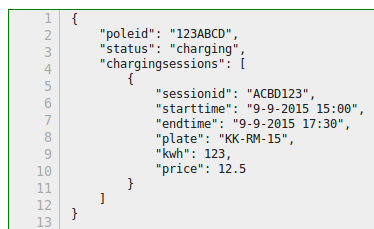
\includegraphics[width=\linewidth]{datastructure.png}
        \end{figure}
    \end{column}
\end{columns}
\end{frame}

%dia 3: backend (UI + API, QUEUES en Workers
\begin{frame}
\frametitle{Backend architecture}
\begin{columns}
    \begin{column}{.5\textwidth}
        \begin{itemize}
            \item Load balancing with weave (or similar)
            \item UI + API: scala + bootstrap
            \item Workers: java or scala
            \item Connected by a queue: RabbitMQ
            \item Can scale with both UI and Worker servers
        \end{itemize}
    \end{column}
    \begin{column}{.5\textwidth}
        \begin{figure}
        \centering
        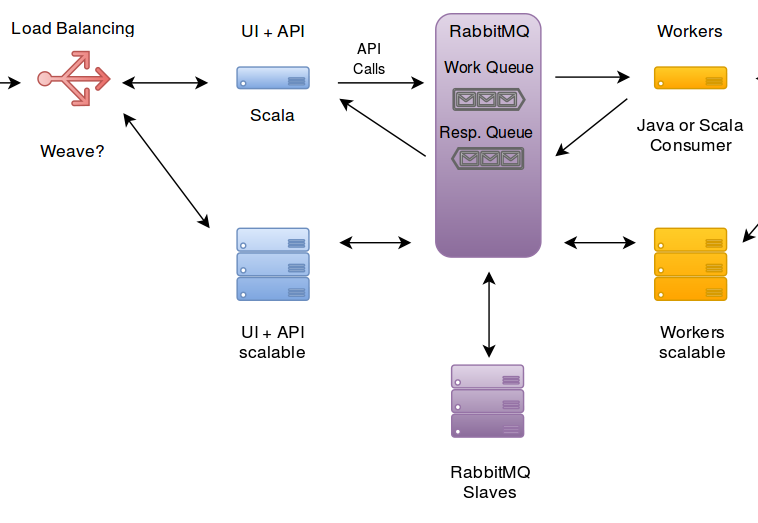
\includegraphics[width=\linewidth]{backend.png}
        \end{figure}
    \end{column}
\end{columns}
\end{frame}

%dia 4: mongodb cluster
\begin{frame}
\frametitle{Database}
\begin{columns}
    \begin{column}{.5\textwidth}
        \begin{itemize}
            \item MongoDB
            \item Using master slave replication or shard cluster
        \end{itemize}
    \end{column}
    \begin{column}{.5\textwidth}
        \begin{figure}
        \centering
        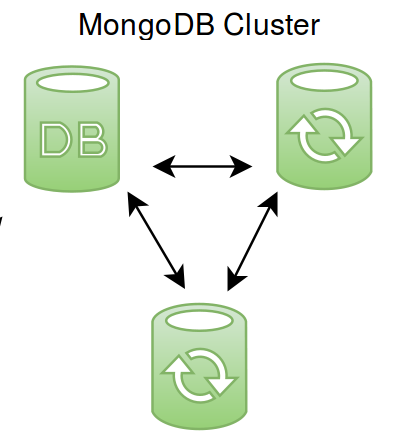
\includegraphics[width=\linewidth]{database.png}
        \end{figure}
    \end{column}
\end{columns}
\end{frame}

%dia 5: totaal plaatje
\begin{frame}
\frametitle{Overview}
\begin{figure}
\centering
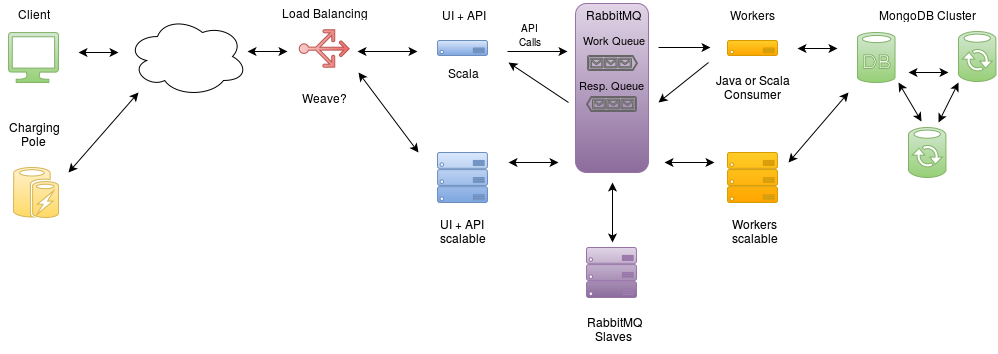
\includegraphics[width=\linewidth]{architecture3.png}
\end{figure}
\end{frame}


\end{document}
